\documentclass{JBCS}

% \usepackage[T1]{fontenc}
\usepackage{graphicx}
% \usepackage{subfigure}
\usepackage{url}
\usepackage{subfig}
\usepackage[brazil]{babel}   
\usepackage[utf8]{inputenc}  
\usepackage{tikz}
\usepackage{amsmath}
\usepackage{amssymb}
\usepackage{cite}
% \usepackage[T1]{fontenc}
% \usepackage[portugues, ruled, lined, linesnumbered]{algorithm2e}

\newcommand{\dtrack}{\textsc{dtrack}}
\newcommand{\rmprt}{{Re\-map\-Rou\-te}}
\newcommand{\figstr}{figura}
\newcommand{\secstr}{seção}
\newcommand{\secstrs}{seções}

\hyphenation{re-map-rou-te}
\hyphenation{Re-map-Rou-te}

% \sloppy
% \newfont{\cunhaemail}{phvr8t at 8.5pt}

\begin{document} 

\setcounter{page}{01}

\cabnames{\'{I}. Cunha, R. Teixeira, D. Veitch e C. Diot}
\cabtit{Remapeando Mudanças de Rota na Internet}

\title{RemapRoute: Remapeando Mudanças de Rota na Internet}
\thankstitle{}

\namea{\'{I}talo Cunha$^1$\quad{}Renata Teixeira$^2$\quad{}Darryl
Veitch$^3$\quad{}Christophe Diot$^4$\vspace{2mm}}

\addressa{$^1$ Departamento de Ciência da Computação, Universidade Federal
de Minas Gerais\\
$^2$ INRIA\\
$^3$ Department of Electrical and Electronic Engineering, University of
Melbourne\\
$^4$ Technicolor}

\nameb{}
\addressb{}

\namec{}
\addressc{}

\named{}
\addressd{}


\maketitle

% \selectlanguage{american}
% 
% \begin{abstract}
% %
% Internet topology maps collected with traceroute may be incomplete or
% out-of-date because we cannot measure frequently enough to detect all
% routing changes without overloading the network.  In this paper, we show
% that routing changes usually affect few routers.  We exploit this
% property to design \rmprt{}, a tool to locally remap Internet routing
% changes that probes only the few affected routers instead of the whole
% route.  Our evaluation with trace-driven simulations and a deployment
% shows that \rmprt{} significantly reduces the number of probes needed to
% remap routes, with no impact on remapping accuracy or latency.  This
% reduction in remapping cost allows us to build more complete and
% up-to-date topology maps.
% %
% \end{abstract}

\begin{abstract} 
%
Mapas topológicos da Internet coletados com traceroute podem estar
incompletos ou desatualizados porque não podemos realizar medições em
frequência suficiente para detectar todas as mudanças de rota.  Neste
artigo mostramos que mudanças de rota geralmente afetam poucos
roteadores.  Exploramos essa propriedade no \rmprt{}, nossa ferramenta
para remapeamento local de mudanças de roteamento que sonda apenas os
poucos roteadores afetados ao invés de toda a rota.  Nossa avaliação via
simulação e um protótipo real mostra que \rmprt{} reduz
significativamente o número de sondas de remapeamento, sem comprometer a
exatidão e a latência de remapeamento.  Esta redução do custo de
remapeamento nos propicia construir mapas topológicos mais completos e
atualizados.
%
\end{abstract}

\keywords{Internet, mapeamento, monitoramento, mudanças de roteamento}

\setcounter{footnote}{0}

\section{Introdução}
\label{sec:intro}

Sistemas para identificação de falhas na Internet coletam medições
frequentes de rotas na rede \cite{duffield06binary,
dhamdhere07netdiagnoser, kompella07blackholes, bassett12lifeguard}.  De
forma similar, redes de distribuição de conteúdo medem rotas na Internet
para escolher o melhor servidor para atender uma requisição
\cite{akamai}.  Esses e outros sistemas medem rotas frequentemente na
esperança de rastrear mudanças de roteamento à medida que elas
acontecem.  

Medições de rota na Internet são frequentemente coletadas com traceroute
\cite{jacobson1989traceroute, augustin07, veitch09balancer}, que envia
sondas para identificar uma sequência de roteadores entre uma origem e
um destino.  A banda disponível para enviar sondas é finita.  Medir
rotas para mapear a topologia requer um grande número de sondas e pode
levar de vários minutos a alguns dias \cite{cunha11fastmapping,
sherwood08discarte, skitter}.  É impossível medir com frequência
suficiente para detectar todas as mudanças de roteamento sem
sobrecarregar a rede.  Consequentemente, mapas da topologia da Internet
podem estar desatualizados ou inconsistentes pois mudanças de roteamento
podem acontecer durante o processo de medição.

Nosso sistema \dtrack{} rastreia mudanças de roteamento na Internet para
manter mapas da topologia da Internet mais atualizados
\cite{cunha11dtrack}.  O \dtrack{} separa as tarefas de detectar e
remapear mudanças de roteamento.  Para detectar mudanças, o \dtrack{}
usa um processo de sondagem leve que combina duas ideias: (1)
redirecionar sondas de caminhos estáveis onde mudanças de roteamento são
improváveis para caminhos instáveis onde mudanças são mais prováveis; e
(2) espalhar sondas de forma uniforme na rede para reduzir medições
redundantes.  Para remapear mudanças, o \dtrack{} usa o Paris traceroute
\cite{augustin07, veitch09balancer} para medir a nova rota por inteiro.
O Paris traceroute é uma versão moderna do traceroute capaz de
identificar roteadores que fazem balanceamento de carga.  Usamos o Paris
traceroute por que é impossível inferir mudanças de roteamento de forma
precisa sem informação sobre roteadores que fazem balanceamento de carga
\cite{cunha11fastmapping}.
\looseness=-1

O \dtrack{} mantém um banco de dados com a última rota observada em cada
um dos caminhos monitorados.  Para detectar mudanças, o \dtrack{} envia
uma sonda num ponto $s^\prime$ do caminho e compara a resposta da sonda
com a última rota observada.  Se a resposta da sonda for incompatível
com a última rota observada, e.g., o endereço IP do roteador que enviou
a resposta não pertence à última rota observada, uma mudança é detectada
e o processo de remapeamento é disparado.  Atualmente, o \dtrack{}
remapeia o caminho por inteiro usando o Paris traceroute.  Esta
abordagem garante medição correta da nova rota, mas desperdiça várias
sondas pois mudanças de caminho envolvem poucos roteadores
(\secstr~\ref{sec:char}).  Em particular, esta abordagem ignora duas
informações disponíveis quando o processo de remapeamento é disparado: a
última rota observada e o ponto $s^\prime$ onde a mudança foi detectada.

Neste artigo propomos \rmprt{}, uma ferramenta para reduzir o custo do
remapeamento de mudanças de roteamento na Internet
(seção~\ref{sec:remap}).  Dadas a última rota observada e um ponto onde
uma mudança foi detectada, o \rmprt{} envia sondas em pontos
estratégicos para localizar a mudança e remapeá-la localmente, sem
desperdiçar sondas nos roteadores que não estão envolvidos na mudança.
Nossa avaliação via simulação dirigida por dados reais mostra que
\rmprt{} reduz pela metade o custo do remapeamento de 88\% das mudanças
de roteamento em nossos dados (seção~\ref{sec:sim}).  A redução de custo
é ainda maior em rotas longas ou com roteadores que fazem balanceamento
de carga.  Nossa avaliação de um protótipo do \rmprt{} usando o
PlanetLab confirma nossos resultados via simulação e demonstra a
eficácia da ferramenta (\secstr~\ref{sec:deploy}).  Sumarizando, neste
artigo fazemos as seguintes contribuições:

\begin{itemize}

\item Caracterizamos mudanças de roteamento na Internet e mostramos que
elas envolvem uma fração pequena dos roteadores numa rota
(\secstr~\ref{sec:char});

\item Propomos métodos para localizar e remapear mudanças de roteamento
que reduzem o desperdício de sondas (\secstr~\ref{sec:remap});

\item Mostramos que nossa ferramenta reduz o custo de remapeamento de
mudanças de rota via simulação e em cenários reais
(\secstrs~\ref{sec:sim} e~\ref{sec:deploy}).

\end{itemize}

A economia de sondas no processo de remapeamento de mudanças de
roteamento aumenta o número de sondas disponíveis para mapeamento
topológico.  Podemos utilizar estas sondas para monitorar mais caminhos
na Internet e melhorar a cobertura dos mapas da topologia, ou aumentar a
frequência de sondagem e melhorar o rastreamento de mudanças de
roteamento.  \rmprt{} é mais um passo na construção de mapas da
topologia da Internet mais completos e consistentes.

\section{Definições e fundamentos}
\label{sec:background}

Seguindo a nomenclatura proposta por Paxson \cite{paxson97routing},
chamamos de \emph{caminho virtual} a conectividade entre uma origem e um
destino na Internet.  Em um dado momento, um caminho virtual é
instanciado por uma \emph{rota}.  Devido a mudanças de roteamento, um
caminho pode ser visto como um processo contínuo $C(t)$ que muda de uma
rota a outra ao longo do tempo.  Uma rota é composta de \emph{saltos}
(\emph{hops}) que são instanciados por roteadores.  Saltos são
enumerados a partir da origem e nos referimos a um salto $s$ numa rota
$C(t)$ por $C(t)[s]$.  Uma rota pode ser \emph{simples} se ela tem
apenas uma sequência de roteadores da origem ao destino; ou
\emph{ramificada} se ela tem roteadores que realizam balanceamento de
carga e múltiplas sequências sobrepostas de roteadores da origem ao
destino.  Todos os saltos numa rota simples têm apenas um roteador e
pelo menos um salto numa rota ramificada tem mais de um roteador.
\looseness=-1

Dadas duas medições consecutivas de um caminho nos instantes $C(t_i)$ e
$C(t_{i+1})$, definimos uma \emph{mudança de caminho} como uma sequência
de saltos contíguos no novo caminho que altera o caminho antigo.
Computamos mudanças de caminho minimizando o número de edições (adição,
remoção e substituição de saltos) necessárias para transformar a nova
rota na rota antiga.  Definimos o \emph{salto de divergência} $s_d$ e o
\emph{salto de convergência} $s_c$ de uma mudança como os saltos
imediatamente anterior e posterior aos saltos editados pela mudança,
respectivamente.  Dizemos que o salto de divergência, o salto de
convergência e todos os saltos entre eles estão \emph{envolvidos} na
mudança de roteamento.  Exemplificando, se $C(t_i) = \{a, b, c, d, e, f,
g\}$ e $C(t_{i+1}) = \{a, b, e, x, y, g\}$, temos uma mudança com $s_d =
1$ e $s_c = 2$ (remoção de $c$ e $d$), e outra mudança com $s_d = 2$ e
$s_c = 5$ (troca de $f$ por $x$ e $y$).

\vspace{-5mm}
\section{Caracterização de mudanças de caminhos}
\label{sec:char}

Nesta seção caracterizamos um conjunto de mudanças de caminho reais e
verificamos que mudanças de caminho na Internet afetam poucos
roteadores.

Implantamos o \dtrack{}~\cite{cunha11dtrack} para medir caminhos em 72
monitores no PlanetLab por uma semana a partir de 4 de março de 2011.
Cada monitor escolhe 1.000 destinos aleatoriamente de uma lista com
34.820 destinos alcançáveis escolhidos aleatoriamente na Internet.  Em
cada monitor, configuramos o \dtrack{} para rastrear mudanças nos
caminhos escolhidos enviando 8 sondas por segundo, similar à taxa de
sondagem do DIMES~\cite{shavitt09dimes}.  Em uma semana observamos
1.202.960 mudanças de caminho.  Os caminhos medidos atravessam 7.315
sistemas autônomos e 97\% dos sistemas autônomos de grande
porte~\cite{oliveira08as2tier}.

\begin{figure*}[t]
\begin{center}
\subfloat[Distribuição do número roteadores envolvidos em mudanças de
caminho]{
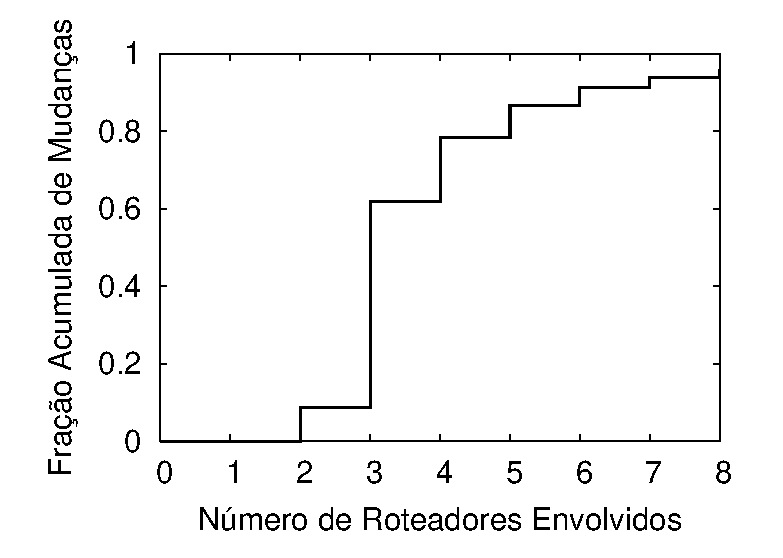
\includegraphics[width=0.94\columnwidth]{figs/nrouters.eps}
\label{fig:char.nrouters}
}
\hspace{5mm}
\subfloat[Distribuição da fração de roteadores de uma rota
envolvidos em mudanças de caminho]{
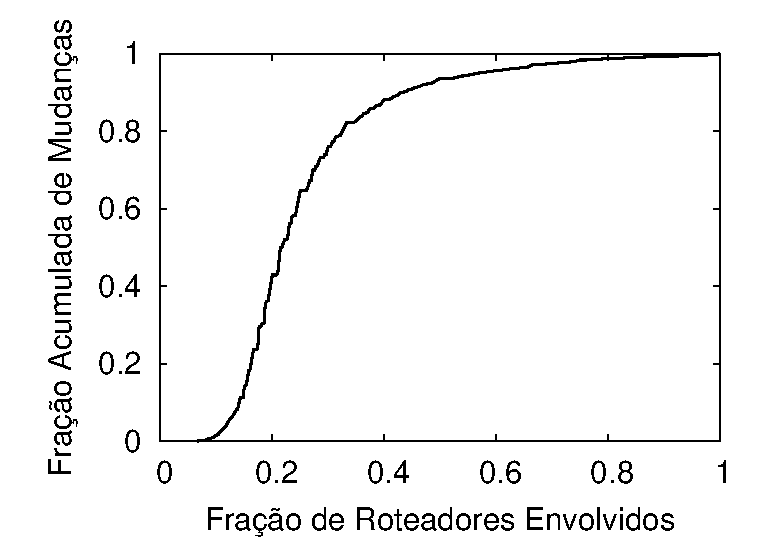
\includegraphics[width=0.94\columnwidth]{figs/fracs.eps}
\label{fig:char.fracs}
}
\caption{Caracterização de mudanças de caminho na Internet}
\label{fig:char}
\end{center}
\end{figure*}

A \figstr~\ref{fig:char.nrouters} mostra a distribuição do número de
saltos envolvidos em mudanças de caminho na Internet.  O número de
saltos envolvidos numa mudança de caminho é o mínimo de saltos que
precisamos remapear para saber qual é a nova rota.  Vemos que 78\% das
mudanças de caminho afetam quatro ou menos saltos, um número pequeno
visto que a mediana do tamanho das rotas em nossos dados é 17 saltos.  O
tipo de mudança de caminho mais comum é quando o roteador de apenas um
salto muda, resultando em mudanças que envolvem três saltos: o salto
onde o roteador mudou mais os saltos de convergência e divergência.
Notamos que 9\% das mudanças de caminho envolvem dois saltos.  Estas
mudanças apenas removem saltos da rota antiga (a nova rota está contida
na rota antiga) e os únicos saltos envolvidos são os saltos de
convergência e divergência.  Causas típicas de mudanças de caminho que
envolvem dois saltos são falhas de conectividade na Internet e erros de
medição onde é impossível medir os saltos atrás da falha ou erro.  

A \figstr~\ref{fig:char.fracs} mostra a distribuição da fração de saltos
de um caminho envolvidos numa mudança, i.e., o número de roteadores
envolvidos na mudança dividido pelo tamanho da nova rota, para todas as
mudanças nos nossos dados.  Vemos que 76\% das mudanças de caminho
envolvem menos de 30\% dos saltos no caminho.  Isso mostra o potencial
do remapeamento local para redução de sondas de medição, se comparado
com a abordagem atual de remapear o caminho por inteiro.  A curva começa
em $x = 0.066 = 2/30$ acontece porque uma mudança envolve pelo menos
dois saltos e porque o \dtrack{} só mede os 30 primeiros saltos num
caminho (o padrão do traceroute e do Paris
traceroute~\cite{jacobson1989traceroute, augustin07}).

A \figstr~\ref{fig:char.nasns} mostra a distribuição do número de
sistemas autônomos envolvidos em mudanças de caminho.  Convertemos
endereços IPs medidos pelo \dtrack{} em sistemas autônomos combinando as
tabelas de mapeamento do Team Cymru\footnotemark{} e
iPlane~\cite{madhyastha06iplane}.  Cada endereço IP que não aparece na
tabela de mapeamento combinada é associado a um sistema autônomo que
contém apenas um endereço IP.  Essa é uma medida conservadora que pode
sobrestimar o número de sistemas autônomos envolvidos em uma mudança.
A \figstr~\ref{fig:char.nasns} explica porque mudanças de roteamento
envolvem poucos saltos.  Mesmo fazendo a conversão de endereços IP para
sistemas autônomos de forma conservadora, vemos que 60\% das mudanças de
caminho é interna a um sistema autônomo e apenas 7\% envolve mais de
dois sistemas autônomos.

\footnotetext{Team Cymru, IP to ASN Mapping,
\url{http://www.team-cymru.org/Services/ip-to-asn.html}}

\begin{figure}[t]
\begin{center}
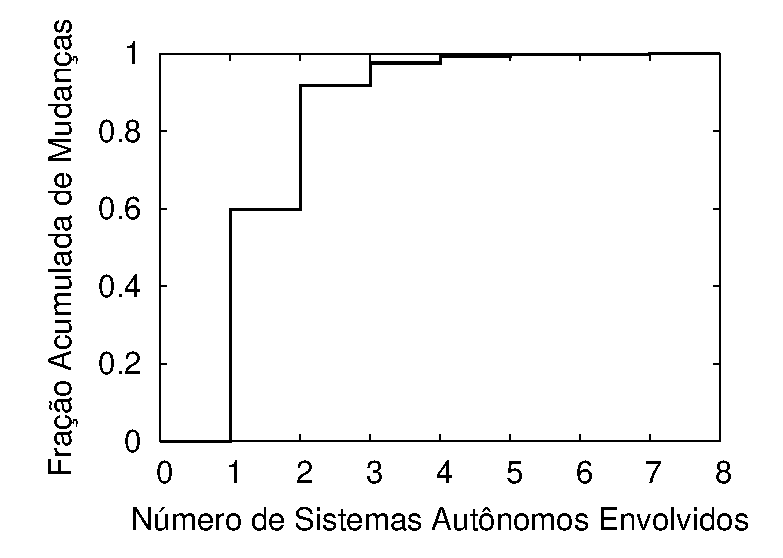
\includegraphics[width=0.96\columnwidth]{figs/nasns.eps}
\caption{Distribuição do número de sistemas autônomos envolvidos em
mudanças de caminho}
\label{fig:char.nasns}
\end{center}
\end{figure}

\section{\textbf{\textsc{RemapRoute}}}
\label{sec:remap}

Agora apresentamos nosso algoritmo para remapeamento local de mudanças
de caminho implementado no \rmprt{}.  O algoritmo recebe como entrada a
rota antiga observada antes da mudança de roteamento $C(t_{i-1})$ e o
salto $s^\prime$ do roteador onde a mudança foi detectada,
$C(t_i)[s^\prime] \ne C(t_{i-1})[s^\prime]$.  Para remapear a mudança de
rota, \rmprt{} opera em duas etapas: primeiro ele localiza onde a
mudança aconteceu (\secstr~\ref{sec:remap.locate}) e depois faz o
remapeamento local da mudança (\secstr~\ref{sec:remap.local}).

O processo de localização e remapeamento da mudança de rota envolve
remapear saltos da rota atual e compará-los com saltos na rota antiga.
Para remapear cada salto, o \rmprt{} envia múltiplas sondas, modificando
sistematicamente os campos do cabeçalho IP como o Paris
traceroute~\cite{augustin07, veitch09balancer}, para identificar
roteadores que fazem balanceamento de carga.

\begin{figure*}[t]
\begin{center}
\begin{tikzpicture}
\draw (-1-0.5,-0.5) -- (-1-0.5,0.5) -- (-1+0.5,0.5) -- (-1+0.5,-0.5) --
cycle;
\node at (-1,0) {O};
%
\draw (10-0.5,-0.5) -- (10-0.5,0.5) -- (10+0.5,0.5) -- (10+0.5,-0.5) --
cycle;
\node at (10,0) {D};
%
\draw (1,0) circle (3mm);
\draw (2,0) circle (3mm);
\draw (3,0) circle (3mm);
\draw[dotted, very thick] (4,0) circle (3mm);
\draw (5,0) circle (3mm);
\draw (6,0) circle (3mm);
\draw (7,0) circle (3mm);
\draw (8,0) circle (3mm);
\node at (1,0) {a};
\node at (2,0) {b};
\node at (3,0) {c};
\node at (4,0) {d};
\node at (5,0) {e};
\node at (6,0) {f};
\node at (7,0) {g};
\node at (8,0) {h};
%
\foreach \i in {1,...,2}
{ \draw (\i+0.3,0) -- (\i+1-0.3,0); }
\foreach \i in {5,...,7}
{ \draw (\i+0.3,0) -- (\i+1-0.3,0); }
\draw[dotted, very thick] (3+0.3,0) -- (4-0.3,0);
\draw[dotted, very thick] (4+0.3,0) -- (5-0.3,0);
\draw (-1+0.5,0) -- (1-0.3,0);
\draw (8+0.3,0) -- (10-0.5,0);
%
\draw[dashed, thick] (3.5,-1) circle (3mm);
\draw[dashed, thick] (4.5,-1) circle (3mm);
\node at (3.5,-1) {x};
\node at (4.5,-1) {y};
\draw[dashed, thick] (3.2,-0.2) -- (3.4,-0.8);
\draw[dashed, thick] (4.8,-0.2) -- (4.6,-0.8);
\draw[dashed, thick] (3.5+0.3,-1) -- (4.5-0.3,-1);
%
\node at (3, 0.5) {$s_d$};
\node at (5, 0.5) {$s_c$};
\node at (7, 0.5) {$s^\prime$};
%
\draw (-2,-1) -- (0,-1) node[right] {ambas as rotas};
\draw[dashed, thick] (-2,-1.5) -- (0,-1.5) node[right] {rota atual};
\draw[dotted, very thick] (-2,-2) -- (0,-2) node[right] {rota antiga};
%
\end{tikzpicture}
\end{center}
\vspace{-4mm}
\caption{Exemplo de mudança de roteamento com adição de roteadores à
rota.}
\label{fig:remap.example}
\end{figure*}

\subsection{Localização da mudança de roteamento}
\label{sec:remap.locate}

O \rmprt{} parte de um salto $s^\prime$ onde o roteador na rota atual é
diferente do roteador na rota antiga, $C(t_i)[s^\prime] \ne
C(t_{i-1})[s^\prime]$.  Se o roteador da rota atual no salto $s^\prime$
não pertencer à rota antiga, $C(t_i)[s^\prime] \notin C(t_{i-1})$, então
$s^\prime$ é um dos saltos envolvidos na mudança de caminho e podemos
passar para a próxima etapa para remapear a mudança
(\secstr~\ref{sec:remap.local}).

Se o roteador da rota atual no salto $s^\prime$ pertencer à rota antiga
em outro salto $s^{\prime\prime}$, $C(t_i)[s^\prime] =
C(t_{i-1})[s^{\prime\prime}]$, então temos uma mudança de roteamento em
saltos anteriores a $s^\prime$ que adicionou ou removeu roteadores na
rota.  A \figstr~\ref{fig:remap.example} mostra um exemplo de uma
mudança de roteamento onde o roteador $d$ foi substituído por dois
roteadores $x$ e $y$.  Uma sonda para o sétimo salto detecta uma mudança
de roteamento pois a resposta da sonda vem do roteador $g = C(t_i)[7]$,
que não é a resposta esperada na rota antiga, $h = C(t_{i-1})[7]$.

Para encontrar um roteador envolvido na mudança de caminho, i.e., um
roteador na rota atual que não está presente na rota antiga, o \rmprt{}
faz uma busca binária no caminho.  O \rmprt{} inicializa $s_\mathrm{esq}
= 0$ e $s_\mathrm{dir} = s^\prime$.  A cada iteração da busca, o
\rmprt{} remapeia o salto $s = (s_\mathrm{esq} + s_\mathrm{dir})/2$ e
procura o roteador no salto $s$ da rota atual na rota antiga.  Se o
roteador no salto $s$ da rota atual não pertencer à rota antiga,
$C(t_i)[s] \notin C(t_{i-1})$, a busca termina e passamos para a etapa
de remapeamento.  Se o roteador no salto $s$ da rota atual estiver no
salto $s$ da rota antiga, $C(t_i)[s] = C(t_{i-1})[s]$, então a mudança
está à direita de $s$ e fazemos $s_\mathrm{esq} = s$.  Se o roteador no
salto $s$ da rota atual estiver em outro salto $s^{\prime\prime}$ na
rota antiga, $C(t_i)[s] = C(t_{i-1})[s^{\prime\prime}]$, a mudança está
à esquerda de $s$ e fazemos $s_\mathrm{dir} = s$.

Não temos como comparar a rota atual com a rota antiga se o roteador no
salto $s$ não responde a sondas.  Neste caso tomamos a decisão
conservadora de decrementar $s$ e continuar a busca no salto anterior,
sem alterar $s_\mathrm{esq}$ e $s_\mathrm{dir}$.  

Se uma mudança de caminho apenas remove saltos da rota antiga, então não
existe salto na rota atual que não pertença à rota antiga.  Neste caso,
o processo de busca termina com $s_\mathrm{esq} = s_\mathrm{dir} + 1$ e
nenhum remapeamento é necessário (\secstr~\ref{sec:remap.local}).

\subsection{Remapeamento local}
\label{sec:remap.local}

O remapeamento local parte de um salto $s$ onde o roteador na rota atual
não pertence à rota antiga, $C(t_i)[s] \notin C(t_{i-1})$.  O \rmprt{}
remapeia sequencialmente os saltos da rota atual posteriores a $s$ até
encontrar o salto de convergência $s_c > s$ com um roteador que pertence
à rota antiga, $C(t_i)[s_c] \in C(t_{i-1})$.  Se uma das rotas não chega
até o destino, o salto de convergência pode não existir.  Neste caso, o
\rmprt{} remapeia a rota atual até o destino ou até o último salto
alcançável.  Se o caminho não chega até o destino, o \rmprt{} identifica
o último salto alcançável após encontrar três saltos consecutivos que
não respondem a sondas (igual o traceroute).

De forma similar, o \rmprt{} remapeia sequencialmente os saltos da rota
atual anteriores a $s$ até encontrar o salto de divergência $s_d < s$
com um roteador que pertence à rota antiga, $C(t_i)[s_d] \in
C(t_{i-1})$.  No pior caso, a busca pelo salto de divergência termina na
origem, que pertence a qualquer rota no caminho.  Se o salto $s_d$ não
for idêntico nas duas rotas, $C(t_i)[s_d] \ne C(t_{i-1})[s_d]$, então
existe outra mudança de roteamento anterior a $s_d$ e voltamos à
primeira etapa (\secstr~\ref{sec:remap.locate}), fazendo $s^\prime =
s_d$, para localizá-la e depois remapeá-la.  Esse processo é realizado
recursivamente até que não reste nenhuma mudança para remapear.
%
O remapeamento dos roteadores nos saltos entre $s_d$ e $s_c$ precisa ser
sequencial pois todos estão envolvidos na mudança de roteamento.  Para
mudanças de roteamento que apenas removem saltos, temos $s_d =
s_\mathrm{esq}$ e $s_c = s_\mathrm{dir}$ e nenhum remapeamento é
necessário.

\vspace{-3mm}
\subsection{Exemplo}

Considere que a mudança de roteamento mostrada na
\figstr~\ref{fig:remap.example} tenha sido detectada com uma sonda para
o quinto salto no caminho.  Temos $C(t_{i-1})[5] = f$ e $C(t_i)[5] = e$.
Como $e \in C(t_{i-1})$, um nó foi inserido antes do quinto salto e o
\rmprt{} inicia uma busca binária para identificar o local da mudança.
O \rmprt{} começa remapeando o segundo salto, onde $C(t_{i-1})[2] =
C(t_i)[2] = c$, indicando que a inserção foi realizada entre o segundo e
o quinto salto.  O \rmprt{} remapeia então o terceiro salto, onde
$C(t_{i-1})[3] = d$ e $C(t_i)[3] = x$.  Como $x \notin C(t_{i-1})$ o
\rmprt{} passa para a fase de remapeamento local da mudança, onde
remapeia o quarto salto e termina.
\looseness=-1

\begin{figure}[t]
\begin{center}
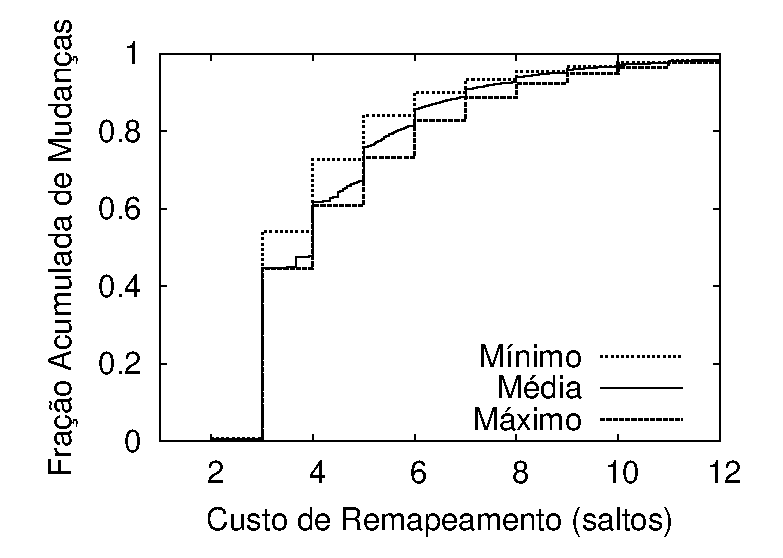
\includegraphics[width=0.96\columnwidth]{figs/rmprtcost.eps}
\caption{Custo de remapeamento com \rmprt{} variando o salto
$\boldsymbol{s^\prime}$ de detecção da mudança.}
\label{fig:sim.rmprt.start}
\end{center}
\end{figure}

\begin{figure*}[t]
\begin{center}
\subfloat[Custo de remapeamento]{
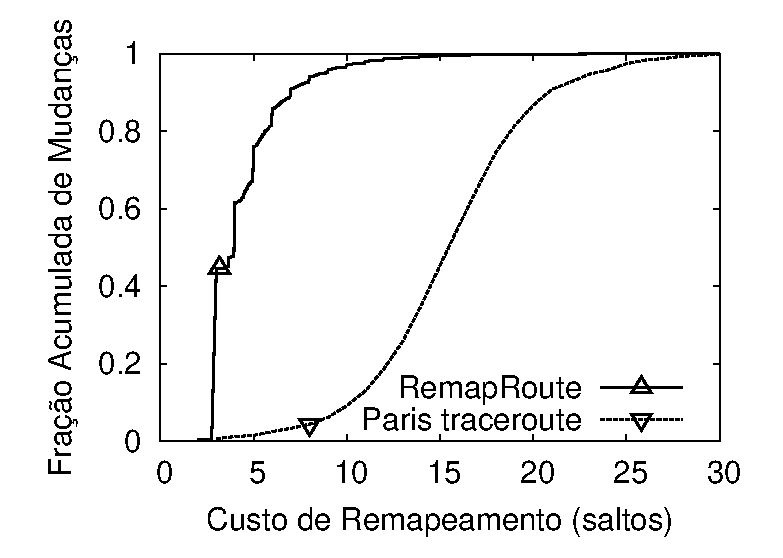
\includegraphics[width=0.94\columnwidth]{figs/costcmp.eps}
\label{fig:sim.abs.cmp}
}
\hspace{5mm}
\subfloat[Redução relativa do custo de remapeamento]{
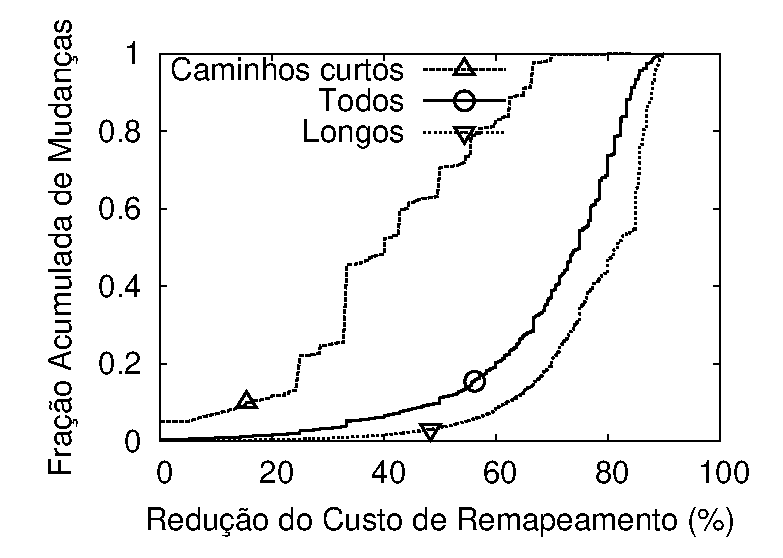
\includegraphics[width=0.94\columnwidth]{figs/lensavings.eps}
\label{fig:sim.savings.cmp}
}
\caption{Comparação do custo de remapeamento entre \rmprt{} e Paris
traceroute.}
\end{center}
\end{figure*}

\section{Avaliação via simulação com dados reais}
\label{sec:sim}

Nesta seção avaliamos o \rmprt{} usando simulações dirigidas com dados
reais.  Utilizamos o mesmo conjunto de dados descrito na
\secstr~\ref{sec:char}.  Nosso foco é comparar o custo de remapear
mudanças de caminho usando o Paris traceroute com o custo de remapear
usando o \rmprt.

O custo de remapeamento usando o \rmprt{} varia de acordo com o salto
$s^\prime$ onde a mudança é detectada.  Calculamos o custo de
remapeamento do \rmprt{} para todos os saltos do caminho onde a mudança
pode ser detectada.  A \figstr~\ref{fig:sim.rmprt.start} mostra a
distribuição do custo de remapeamento de mudanças para o \rmprt{}.
Mostramos a distribuição dos custos mínimo, médio e máximo, calculados
sobre todos os saltos envolvidos em uma mudança.  Vemos que o custo
mínimo e máximo em geral são muito próximos.  Uma razão para este
comportamento é que várias mudanças de caminho envolvem poucos
roteadores, logo não existe muita variação em função do salto $s^\prime$
onde a mudança é detectada.  No resto deste artigo usaremos o custo
médio como representativo do custo de remapeamento com \rmprt{}.

A \figstr~\ref{fig:sim.abs.cmp} compara o custo de remapeamento do
\rmprt{} com o custo de remapeamento do Paris traceroute.  Comparando
com a \figstr~\ref{fig:char.nrouters} vemos que o \rmprt{}
frequentemente precisa sondar um número de saltos maior do que o número
de saltos envolvidos numa mudança.  Este aumento deve-se a mudanças de
roteamento que precisam ser localizadas usando a técnica de pesquisa
binária antes de serem remapeadas.  Independente do processo de
localização, o \rmprt{} tem custo de remapeamento significativamente
menor que o do Paris traceroute.  Note que o custo de remapeamento do
\rmprt{} raramente é menor do que três saltos, mesmo com 9\% das
mudanças envolvendo apenas dois saltos
(\figstr~\ref{fig:char.nrouters}).  As mudanças que envolvem apenas dois
roteadores apenas removem saltos da rota antiga, e precisamos localizar
o salto onde a remoção aconteceu usando busca binária.  A busca binária
requer pelo menos três sondas a não ser que a mudança seja detectada nos
três primeiros saltos do caminho, o que acontece em 0,4\% das mudanças
em nossos dados.

A \figstr~\ref{fig:sim.savings.cmp} mostra a distribuição da redução no
custo de remapeamento quando usamos \rmprt{} em vez do Paris traceroute.
Calculamos a redução do custo de remapeamento como $(C_\mathrm{Paris} -
C_\mathrm{\rmprt})/C_\mathrm{Paris}$, onde $C_\mathrm{Paris}$ é o número
de saltos remapeados pelo Paris traceroute e $C_\mathrm{\rmprt}$ é o
número de saltos remapeados pelo \rmprt{}.  A linha sólida, calculada
para todas as mudanças de caminho em nossos dados, mostra que a redução
no custo é significativa.  O \rmprt{} reduz pra menos da metade o custo
de remapeamento de 88\% das mudanças de caminho.  As linhas tracejadas
na \figstr~\ref{fig:sim.savings.cmp} mostram a redução no custo para
mudanças em rotas menores que 10 saltos (curtas) e maiores que 20 saltos
(longas).  Vemos que a redução no custo é mais acentuada para rotas
longas, onde o Paris traceroute desperdiça sondas em vários roteadores
que não estão envolvidos na mudança, e que o \rmprt{} traz redução de
custos para remapeamento mesmo em rotas curtas.

\subsection{Erros de remapeamento}

O \rmprt{} remapeia mudanças num caminho dado um salto $s^\prime$ onde
uma mudança foi detectada.  Isso pode levar a inconsistências caso um
caminho sofra duas ou mais mudanças disjuntas antes de detectarmos a
primeira mudança.  Por exemplo, um caminho $\{a, b, c, d, e, f, g\}$
pode mudar para $\{a, x, c, d, y, f, g\}$ entre duas medições
consecutivas com Paris traceroute.  Neste caso, podemos detectar duas
mudanças nos saltos $s^\prime = 1$ e $s^{\prime\prime} = 4$.
Infelizmente, dado $s^\prime$ ou $s^{\prime\prime}$, o \rmprt{}
remapeará apenas uma mudança.

Para avaliar a gravidade desse problema, a
\figstr~\ref{fig:sim.ndisjoint} mostra a distribuição do número de
mudanças disjuntas para os pares de medições consecutivas dos caminhos
em nosso conjunto de dados.\footnotemark{}  Vemos que 79\% das medições
consecutivas remapeiam apenas uma mudança disjunta, que o \rmprt{}
remapeará corretamente para qualquer salto $s^\prime$ onde a mudança for
detectada.  Apenas 3\% das medições consecutivas remapeiam três ou mais
mudanças disjuntas, indicando que o \rmprt{} remapeará a nova rota
corretamente na maioria dos casos.

\footnotetext{No nosso conjunto de dados só medimos caminhos com Paris
traceroute quando uma mudança é detectada.  Todos os pares de medições
consecutivas remapeiam pelo menos uma mudança disjunta.}

\begin{figure}
\begin{center}
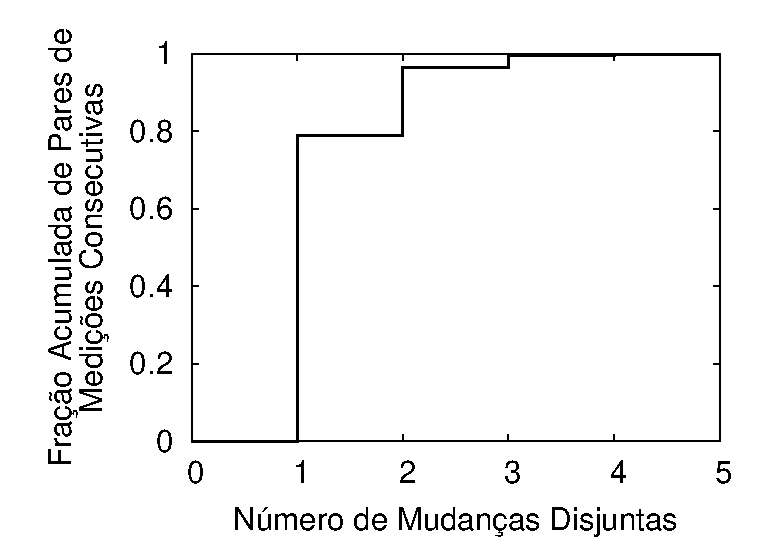
\includegraphics[width=0.96\columnwidth]{figs/ndisjoint.eps}
\caption{Distribuição do número de mudanças disjuntas entre duas
medições com Paris traceroute.}
\label{fig:sim.ndisjoint}
\end{center}
\end{figure}

Três outros fatores contribuem para minimizar o impacto de mudanças
disjuntas.  Primeiro, o \rmprt{} pode remapear mudanças disjuntas
anteriores ao salto de detecção $s^\prime$ caso ele as detecte durante o
processo de remapeamento.  Em particular, a probabilidade do \rmprt{}
remapear uma mudança disjunta anterior ao salto de detecção $s^\prime$
no nosso conjunto de dados é 43\%.  Segundo, uma mudança disjunta que
não for remapeada quando executarmos \rmprt{} será detectada e remapeada
no futuro (assumindo que o processo de sondagem para detecção de
mudanças de caminho seja capaz de detectar todas as mudanças possíveis).
Qualquer mudança disjunta que não for remapeada causa apenas uma
inconsistência temporária nos dados.  Terceiro, a redução do custo de
remapeamento obtida com \rmprt{} pode ser utilizada para aumentar a
frequência de sondagem para detecção de mudanças e reduzir a chance de
ocorrerem duas mudanças em um caminho antes de detectarmos a primeira.
\looseness=-1

Outra limitação do \rmprt{} é que o mecanismo de busca binária pode
falhar quando a ordem relativa de dois saltos se inverte da rota antiga
para a nova rota.  Um exemplo extremo, mas ilustrativo, é uma mudança de
$C(t_{i-1}) = \{a, b, c, d, e, f\}$ para $C(t) = \{a, e, d, c, b, f\}$.
Apenas 0,9\% das mudanças de caminho em nossos dados invertem a ordem
relativa de saltos.  Como inversão da ordem relativa de saltos é um
evento raro, tomamos a decisão conservadora de remapear o caminho por
inteiro (como o Paris traceroute) quando uma inversão é detectada
durante o processo de remapeamento.  Como mostram os resultados
anteriores, essa limitação não compromete a utilidade do \rmprt{}.

\section{Avaliação com protótipo real no PlanetLab}
\label{sec:deploy}

Nesta seção avaliamos um protótipo do \rmprt{} no PlanetLab.
Implantamos o Paris traceroute e o \rmprt{} em 140 nós PlanetLab e
coletamos medições por 18 horas de 30 de Novembro de 2012.  Cada nó
executa o Paris traceroute para medir caminhos periodicamente.  Como no
conjunto de dados utilizado nas seções anteriores, cada nó monitora
caminhos para 1.000 destinos escolhidos aleatoriamente de uma lista com
34.820 destinos alcançáveis na Internet.  Quando duas medições
consecutivas com Paris traceroute detectam uma mudança, executamos o
\rmprt{} para remapeá-la.  Cada nó leva em média 7~horas e 42~minutos
para medir os 1.000 caminhos.  Devido à baixa frequência de sondagem,
este conjunto de dados contém apenas 87.848 mudanças.  Os caminhos
medidos atravessam 7.143 sistemas autônomos e 95\% dos sistemas
autônomos de grande porte na Internet~\cite{oliveira08as2tier}.
\looseness=-1

\begin{figure}
\begin{center}
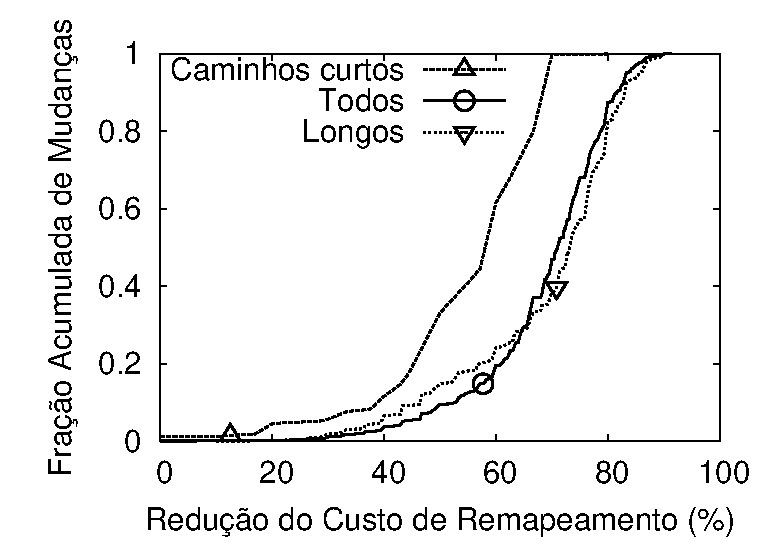
\includegraphics[width=0.96\columnwidth]{figs/deploysavings.eps}
\caption{Redução do custo de remapeamento com \rmprt{} em cenários
reais.}
\label{fig:deploy.savings}
\end{center}
\end{figure}

\begin{figure*}
\begin{center}
\subfloat[\rmprt{}]{
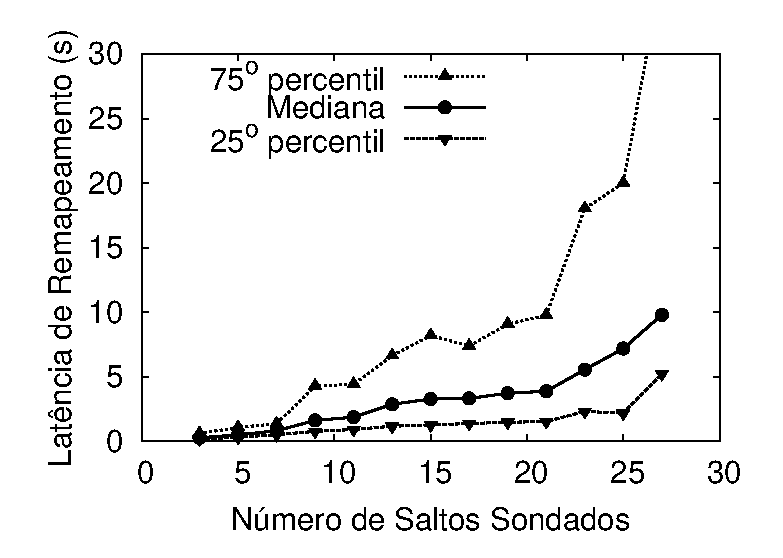
\includegraphics[width=0.94\columnwidth]{figs/latency.eps}
\label{fig:deploy.latency}
}
\hspace{5mm}
\subfloat[Paris traceroute]{
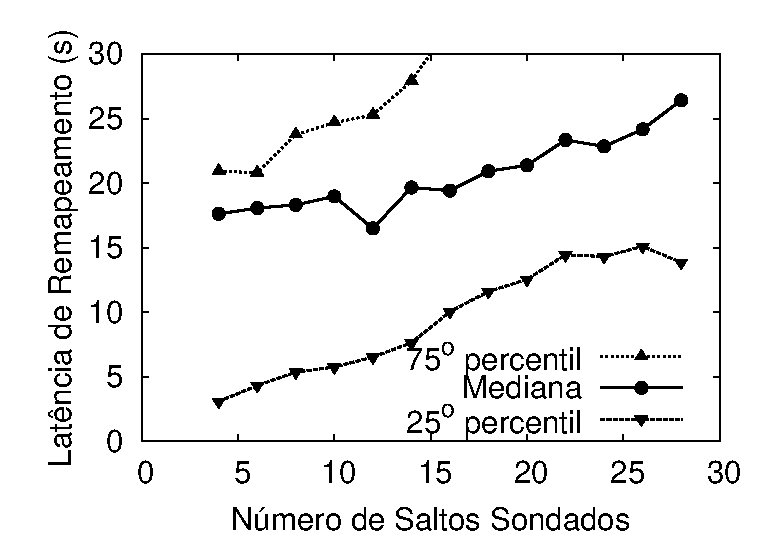
\includegraphics[width=0.94\columnwidth]{figs/ptrlatency.eps}
\label{fig:deploy.latency.ptr}
}
\caption{Latência de remapeamento em cenários reais.}
\end{center}
\end{figure*}

A \figstr~\ref{fig:deploy.savings} mostra a redução do custo de
remapeamento quando usamos o \rmprt{} em vez do Paris traceroute.
Comparando com a \figstr~\ref{fig:sim.savings.cmp}, a redução média do
custo de remapeamento no cenário real é quantitativamente similar aos
resultados obtidos via simulação (linha sólida).  Por exemplo, reduzimos
pra menos da metade o custo de remapeamento de 90\% das mudanças de
caminho no cenário real.

A redução de custo para rotas curtas e longas é mais similar à redução
de custo geral no cenário real que nas simulações.  Em outras palavras,
as linhas tracejadas na \figstr~\ref{fig:deploy.savings} estão mais
próximas da linha sólida que na \figstr~\ref{fig:sim.savings.cmp}.
Atribuímos essa mudança a três fatores: (i) o menor número de mudanças
observadas no cenário real pode limitar a variedade de mudanças
observadas; (ii) diferenças no conjunto de caminhos monitorados; e (iii)
a diferente forma de detecção de mudanças (os dados utilizados nas
simulações foram coletados com o \dtrack{}).

A \figstr~\ref{fig:deploy.latency} mostra os $25^o$, $50^o$ e o $75^o$
percentis da latência de remapeamento em função do número de saltos
sondados durante o processo de remapeamento.  Avaliamos a latência de
remapeamento por que o \rmprt{} sonda saltos sequencialmente: a decisão
do próximo salto a sondar depende do resultado do último salto sondado.
O Paris traceroute, em contrapartida, poderia paralelizar a sondagem de
saltos (apesar da implementação padrão não fazê-lo).  Como a maior parte
dos remapeamentos com \rmprt{} requer sondagem de poucos saltos
(\figstr~\ref{fig:sim.abs.cmp}), a latência de remapeamento geralmente é
menor que 5 segundos.  A \figstr~\ref{fig:deploy.latency.ptr} mostra os
$25^o$, $50^o$ e $75^o$ percentis da latência de remapeamento com Paris
traceroute no cenário real.  Nosso objetivo não é comparar a latência de
remapeamento do \rmprt{} com Paris traceroute, pois a latência é
diretamente afetada por decisões de implementação da ferramenta.  Nosso
objetivo é mostrar que a latência de remapeamento com \rmprt{} é
aceitável para uso em sistemas reais.  Notamos ainda que um sistema de
mapeamento topológico como o \dtrack{} pode executar o \rmprt{}
simultaneamente em caminhos diferentes caso mais de uma mudança seja
detectada num curto intervalo de tempo.

Por último, avaliamos se o remapeamento com o \rmprt{} é equivalente a
utilizar o Paris traceroute para medir o novo caminho por inteiro.  Para
cada mudança observada no cenário real, comparamos os saltos remapeados
pelo \rmprt{} com a rota medida pelo Paris traceroute.  Apenas 0,6\% das
medições com \rmprt{} são diferentes das medições com Paris traceroute.
A identificação de roteadores que fazem balanceamento de carga usando
Paris traceroute ou \rmprt{} é probabilística~\cite{veitch09balancer}.
Por exemplo, a configuração padrão do Paris traceroute e do \rmprt{}
identifica todos os roteadores que fazem balanceamento de carga numa
rota com 95\% de confiabilidade.  Erros de medição são inevitáveis e
causam diferenças entre remapeamentos independente da ferramenta
utilizada.  Outra causa para diferença nos remapeamentos são mudanças de
roteamento que acontecem no intervalo entre a medição com Paris
traceroute e a medição com \rmprt{}.

Sumarizando, o remapeamento de mudanças de caminho na Internet com
\rmprt{} é tão preciso quanto remapeamento com Paris traceroute, reduz
significativamente o número de sondas enviadas e tem pouco impacto na
latência de remapeamento.

\section{Trabalhos relacionados}
\label{sec:related}

Operadores podem utilizar mensagens dos protocolos de roteamento (e.g.,
OSPF e IS-IS) e arquivos de configuração dos roteadores para mapear a
topologia de sua rede~\cite{feamster05nsdi, turner10cenic,
athina08link}.  Esta abordagem resulta em mapas completos e precisos da
topologia, mas só está disponível para operadores de redes e é restrita
a uma única rede.  Para mapear múltiplas redes, podemos utilizar
coletores públicos de mensagens BGP\footnotemark{} para construir um
mapa dos sistemas autônomos da Internet~\cite{oliveira08as2tier,
dhamdhere08evo}.  Infelizmente, o BGP não expõe todos os enlaces da rede
e coletores públicos de mensagens BGP não cobrem todos os sistemas
autônomos da Internet~\cite{oliveira08as2tier, cohen06darkmatter}.
Neste trabalho tomamos a abordagem ortogonal de medir a topologia da
rede no nível de roteadores usando medições ativas.

\footnotetext{The University of Oregon Routeviews Project,
\url{http://www.routeviews.org}\newline{}
RIPE Routing Information Service,
\url{http://www.ripe.net/data-tools/stats/ris}}

Pesquisa sobre mapeamento topológico no nível de roteadores usando
medições ativas têm três objetivos principais: (i) aumentar a cobertura
da Internet, (ii) aumentar a precisão da topologia construída e (iii)
aumentar a frequência das medições.

A abordagem clássica para aumentar a cobertura da Internet é monitorar
um grande número de caminhos.  A plataforma Skitter/Ark da
CAIDA~\cite{skitter} tenta cobrir toda a Internet usando alguns
monitores para medir caminhos para todos os prefixos $/24$ anunciados na
Internet.  O problema é que o Skitter/Ark demora de dois a três dias
para coletar a topologia devido ao grande número de caminhos monitorados
e limitações de banda nos monitores.  Uma alternativa é dividir a carga
de sondagem das medições entre vários monitores, como nos sistemas
DIMES~\cite{shavitt09dimes} e Ono~\cite{choffnes10crowd}.  Neste
trabalho assumimos que o conjunto de monitores e destinos é fixo.
Porém, utilização do RemapRoute é ortogonal ao conjunto de monitores e
destinos.  O RemapRoute pode ser usado por qualquer um dos sistemas
acima para reduzir a sobrecarga de rede.

Técnicas para aumentar a precisão da topologia coletada tentam inferir
mais informações sobre a rede do que medições tradicionais com
traceroute.  O Paris traceroute envia sondas adicionais variando
sistematicamente os valores nos campos do cabeçalho IP para detectar
todos os roteadores que fazem balanceamento de carga em uma
caminho~\cite{augustin07, veitch09balancer}.  O \rmprt{} detecta
roteadores que fazem balanceamento de carga utilizando o mesmo algoritmo
que o Paris traceroute.  O DisCarte usa traceroute e sondas com a opção
\emph{Record Route} do protocolo IP ativada para coletar duas sequências
relacionadas de roteadores em caminhos da
Internet~\cite{sherwood08discarte}.  O DisCarte pós-processa essas
sequências com ferramentas de aprendizado de máquina para combiná-las em
uma topologia mais precisa.  Estas e outras técnicas enviam sondas
adicionais e aumentam o custo de mapeamento da topologia.  O objetivo do
RemapRoute é complementar: reduzir o custo do remapeamento de mudanças
de roteamento, aumentando a disponibilidade de sondas para coleta de
topologias mais precisas.  

Nosso trabalho é mais relacionado com técnicas para aumentar a
frequência de medições da topologia da Internet.  Em geral, monitores
têm banda de rede limitada para mapear a topologia.  Reduzir o custo de
cada medição da topologia aumenta diretamente a frequência com a qual
medições podem ser coletadas.  O RocketFuel, por exemplo, reduz o custo
para mapear a topologia de um sistema autônomo alvo descartando caminhos
que têm roteadores de ingresso e egresso no sistema autônomo alvo
idênticos a outro caminho já medido~\cite{spring02rocketfuel}.  Outra
abordagem é reduzir o custo de medições escolhendo apenas um destino em
cada sub-rede num sistema autônomo~\cite{beverly10hifreq}.  O Doubletree
reduz sondas redundantes nos roteadores próximos a monitores
(compartilhados pelos caminhos partindo do monitor) e nos roteadores
próximos a destinos (compartilhados pelos caminhos que terminam no
destino)~\cite{donnet05topology}.  O \rmprt{} foi desenvolvido para
reduzir o custo do remapeamento de mudanças no \dtrack{}, nosso sistema
de mapeamento topológico~\cite{cunha11dtrack}.  O \rmprt{} e o \dtrack{}
complementam as técnicas existentes para redução do custo de mapeamento
topológico.  O \dtrack{} reduz sondas redundantes para roteadores
próximos aos monitores como o Doubletree e é compatível com técnicas
descritas acima para selecionar quais caminhos mapear.

\section{Conclusões e trabalhos futuros}
\label{sec:conc}

A manutenção de mapas completos e atualizados da Internet é difícil
devido à grande quantidade de sondas necessárias e restrições de banda
nos monitores.  Neste trabalho propomos o \rmprt{}, uma ferramenta para
reduzir o custo de remapeamento de mudanças de roteamento na Internet.
Dadas a rota anterior a uma mudança de roteamento e um salto
(\emph{hop}) onde a mudança foi detectada, o \rmprt{} (1) realiza uma
busca binária pelo salto onde a mudança aconteceu e (2) faz o
remapeamento local da mudança.  Comparado com a abordagem atual de
remapear a nova rota por inteiro usando traceroute, o \rmprt{} reduz
significativamente o número de saltos sondados para remapear mudanças de
roteamento na Internet.  Essa redução de saltos sondados aumenta a
disponibilidade de sondas, potencializando a medição de mais caminhos ou
aumento da frequência de medições.  O remapeamento com \rmprt{} é tão
preciso quanto remapear o caminho inteiro com traceroute, e a latência
de remapeamento é satisfatória para utilização do \rmprt{} em sistemas
reais.  \rmprt{} é mais um passo na construção de mapas da topologia da
Internet mais completos e atualizados.

Como trabalho futuro, pretendemos integrar o \rmprt{} no \dtrack{} e
prover um serviço de mapeamento da Internet aberto para disponibilizar
informações sobre a topologia para pesquisadores e aplicações.  Queremos
também reduzir ainda mais o custo de remapeamento de mudanças no
\dtrack{}.  Atualmente, o \dtrack{} remapeia cada caminho separadamente.
Esta abordagem desperdiça sondas caso vários caminhos sejam afetados
pela mesma mudança.  Pretendemos desenvolver mecanismos para prever
quais caminhos são afetados por uma mesma mudança e remapear apenas um
deles.


\bibliographystyle{plain}
\bibliography{references}

\end{document}
